% ==========================================================================
% prednaska DS 7.4.2003

\chapter{Haldy}

\begin{defn}
Haldy jsou stromové struktury, které splňují 
\begin{itemize}
\item lokální podmínku na uspořádání
  - prvek reprezentující otce je menší než prvek reprezentovaný synem
    apod.
% oprava by M. Macok:
% "strukturalni podminky" na stromy jsou podminky na tvar
% stromu (event. lesu), podle kterejch se ty haldy rozdelujou na Fib.,
% leftlist apod... neni tam nic o tom, jestli jsou synove vetsi/mensi
% nez otcove apod., od toho je tam ta prvni podminka...
\item strukturální podmínku na stromy, ze kterých jsou vytvořené 
\end{itemize}
\end{defn}

\begin{pozn}
Podle těchto podmínek se haldy rozdělují na Fibonacciho, Leftist,
d-regulární apod. (mohou se lišit jak lokální, tak strukturální podmínkou)
\end{pozn}

% --------------------------------------------------------------------------
\section{$d$-regulární haldy}

\begin{defn}
d-regulární halda, $d$ celé číslo $d \geq 2$ \\
Je to strom $T$ takový, že existuje jednoznačná korespondence mezi vrcholy
stromů a prvky reprezentované množiny a platí:
\begin{enumerate}
\item strom $T$ splňuje strukturální podmínky:
  \begin{itemize}
    \item každý vrchol s vyjímkou nejvýše jednoho je buď list nebo má $d$ synů
    \item každý vrchol má nejvýše $d$ synů
    \item existuje očíslování synů každého vrcholu tak, že po očíslování
  	  průchodem do šířky platí: \\
	  když vrchol není list, pak každý vrchol s menším číslem má $d$
	  synů.
	  %\footnote{Tato podmínka říká jinými slovy toto: V poslední
	  %hladině jsou všechny uzly umístěny co možná nejvíce "vlevo",
	  %tzn. procházíme-li uzly předposlední hladiny zleva doprava,
	  %nejprve má několik z nich (popř. žádný) $d$ následníků, pak může
	  %být (ale nemusí) jeden uzel s jedním následníkem a zbývající 
	  %uzly předposlední hladiny následníky
	  %nemají. (parafráze z~\cite{Topfer}, str.~79)}.
  \end{itemize}
  \item podmínku na lokální uspořádání: \\
	když $x$ je prvek přiřazený vrcholu $t$, pak otci($t$) je přiřazen
	prvek $\leq x$ pak po očíslování průchodem do šířky platí:
	když vrchol má číslo $i$, jeho synové mají čísla
% oprava by M.Macok :
% strana 70, prvni syn vrcholu neni na pozici d(i-1)+1 ale ..+2
	$d(i-1)+2,d(i-1)+3,...,di+1$ a otec má číslo 
	$\lceil\frac{i-1}{d}\rceil$.
\end{enumerate}
\end{defn}

\begin{priklad}
Příklad 3-regulární haldy je na obrázku~\ref{XXX}.

\mnote{XXX chybi obr.}

Když takto očíslované prvky dáme do pole, pak platí: když je vrchol na
$i$-tém místě, čísla synů jsou $3(i-1)+2, 3i, 3i+1$
a otec je na $\lceil\frac{i-1}{3}\rceil$ místě v poli.
to využijeme pro implementaci polem - ušetříme místo.
\end{priklad}

\begin{pozn}
Nejpopulárnější jsou 2-reg. haldy, protože synové i-tého vrcholu
jsou na místech $2(i-1)+2=2i, 2(i-1)+3=2i + 1$, otec je na
$\lceil\frac{i-1}{2}\rceil + 1 = \lceil\frac{i}{2}\rceil$. 
$\Rightarrow$ snadné počítání (bitový posun)
\end{pozn}

\subsection{Algoritmus UP}

Operace UP($x$) srovná haldu směrem nahoru.

\begin{algorithm}[!htb]
\caption{UP pro d-regulární haldy}
\label{alg:heap.dreg.up}
\begin{algorithmic}
\STATE A: 
\IF {prvek reprezentovaný $x$ je $<$ prvek reprezentovaný otcem($x$)} 
  \STATE $x$ a otce($x$) vyměníme 
  \STATE pokračujeme v A
\ENDIF
\end{algorithmic}
\end{algorithm}


\subsection{Algoritmus DOWN}

\begin{algorithm}[!htb]
\caption{DOWN pro d-regulární haldy}
\label{alg:heap.dreg.down}
\begin{algorithmic}
\STATE A:
\IF {prvek reprezentovaný $x >$ prvek reprezentovaný některým synem $x$}
  \STATE vyměníme $x$ a syna $x$, který reprezentuje nejmenší prvek,
  \STATE pokračujeme v A
\ENDIF
\end{algorithmic}
\end{algorithm}

\begin{pozn}
Když má hlada hloubku $h$, pak UP($x$) vyžaduje čas $O(h)$, DOWN($x$) čas
$O(dh)$.
\end{pozn}

\subsection{Operace na haldě}

\subsubsection{INSERT}

\begin{algorithm}[!htb]
\caption{INSERT pro d-regulární haldy}
\label{alg:heap.dreg.insert}
\begin{algorithmic}
\STATE přidáme poslední list $t$ reprezentující $x$
\STATE UP($t$)
\end{algorithmic}
\end{algorithm}

\subsubsection{MIN}

\begin{algorithm}[!htb]
\caption{MIN pro d-regulární haldy}
\label{alg:heap.dreg.min}
\begin{algorithmic}
\STATE vrátí prvek reprezentovaný v kořeni
\end{algorithmic}
\end{algorithm}

\subsubsection{DELETEMIN}

viz algoritmus~\ref{alg:heap.dreg.deletemin}.

\begin{algorithm}[!htb]
\caption{DELETEMIN pro d-regulární haldy}
\label{alg:heap.dreg.deletemin}
\begin{algorithmic}
\STATE prvek reprezentovaný posledním listem dáme do kořene
\STATE odstraníme poslední list 
\STATE DOWN(kořen)
\end{algorithmic}
\end{algorithm}

\subsubsection{DECREASEKEY$(x, \Delta)$}

Provedení této operace předpokládá, že musíme znát polohu vrcholu $t$
reprezentujícího $x$, toto halda neumožňuje nalézt. 

viz algoritmus~\ref{alg:heap.dreg.decrkey}.

\begin{algorithm}[!htb]
\caption{DECREASEKEY pro d-regulární haldy}
\label{alg:heap.dreg.decrkey}
\begin{algorithmic}
\STATE změníme uspořádání v bodě $x$ 
\STATE UP($x$) mohl by být menší než jeho otec, proto provedeme UP 
\end{algorithmic}
\end{algorithm}

\subsubsection{INCREASEKEY$(x, \Delta)$}

Musíme znát polohu vrcholu $t$ reprezentujícího $x$, 
toto halda neumožňuje nalézt. 
viz algoritmus~\ref{alg:heap.dreg.incrkey}.

\begin{algorithm}[!htb]
\caption{INCREASEKEY pro d-regulární haldy}
\label{alg:heap.dreg.incrkey}
\begin{algorithmic}
\STATE změníme uspořádání v bodě $x$ 
\STATE DOWN($x$)
\end{algorithmic}
\end{algorithm}

\subsubsection{DELETE}

Musíme znát polohu vrcholu $t$ reprezentujícího $x$, toto halda neumožňuje
nalézt.
\par
Vezmeme prvek $y$ reprezentovaný posledním listem, odstraníme poslední list,
prvek $t$, který reprezentoval $x$ bude reprezentovat $y$.


\begin{algorithm}[!htb]
\caption{DELETE pro d-regulární haldy}
\label{alg:heap.dreg.delete}
\begin{algorithmic}
\IF {$y < x$} 
  \STATE UP($t$) else DOWN($t$) 
\ENDIF
\end{algorithmic}
\end{algorithm}

\subsection{Algoritmus MAKEHEAP}

Dána prostá posloupnost $x_1, x_2, ..., x_n$.
Chceme vytvořit d-reg. haldu reprezentující množinu 
${ x_1, x_2, ..., x_n }$. Vezmeme "d-reg. strom" $T$ s vrcholy přiřadíme
prvky $x_1, x_2, ..., x_n$. Pro všechny vrcholy, které nejsou listy podle
očíslování v pořadí od největšího k nejmenšímu provedeme DOWN($t$).
\par

\mnote{chybí obrázek}
% XXX obr.

Invariant: v okamžiku, kdy provádím DOWN($t$), tak vrcholy, které
reprezentující větší prvky splňují směrem dolů podmínku 

\subsection{Složitost operací}

V d-reg. haldě reprezentující n-prvkovou množinu implementace operací
vyžaduje časy dané tabulkou:

\begin{center}
\begin{tabular}{|l|l|}
\hline
Operace & Složitost \\
\hline
MIN & O(1) \\
INSERT, DECREASEKEY & $O(log_d(n))$ \\
DELETEMIN, INCREASEKEY, DELETE & $O(d \cdot log_d(n))$ \\
\hline
\par
\end{tabular}
\end{center}

Máme vrchol v $i$-té hladině a "d-regulární strom" má hloubku $h$. 
Kolik času potřebuje DOWN($t$) ?
Je to $O(d(h-1))$.
\par
Počet vrcholů v $i$-té hladině je $di$. \\
Čas MAKEHEAP je 
$O(\sum_{i=0}^{h-1} d^id(h-i)) = O(dS)$, kde 
$$
S = \sum_{i=0}^{h-1} d^i(h-i)
$$

Budeme počítat 
\begin{multline}\bigparens
dS - S = \sum_{i=0}^{h-1}d^{i+1}(h-i) - \sum_{i=0}^{h-1}d^{i}(h-i) = \\
d^h - h + \sum_{i=0}^{h-1}d^{i}(h-i-(h-i-1)) = d^h - h\frac{d^h - 1}{d-1} \\
\Rightarrow S = \frac{d^h - h}{d-1} + d\frac{d^{h-1} - 1}{(d-1)^2}, 
h = log_d(n) \Rightarrow S \approx O(\frac{n}{d})
\end{multline}


\subsection{Dijkstrův algoritmus}

K čemu jsou d-reg. haldy dobré ? např. pro implementaci Dijkstrova
algoritmu.
\par

\begin{itemize}
\item[Vstup:] orientovaný graf $(V,E)$, fce $c:E \rightarrow R^+$, vrchol $z$
\item[Výstup:] $d(v)$, $v \in V$ \\
	$d(v)$ je délka nejkratší cesty ze $z$ do $v$ \\
\end{itemize}

\begin{algorithm}[!htb]
\caption{Dijkstrův algoritmus pro d-regulární haldy}
\label{alg:heaps.d-reg.dijkstra}
\begin{algorithmic}
\STATE $d(z) = 0, d(v) = \infty \forall v \in V, v \neq z, U = {z}$\\
\WHILE {$U \neq \emptyset$}
  \STATE vezmeme z $U$ prvek $u \in U$ s nejmenší hodnotou $d(u)$,
    \STATE odstraníme ho z $U$.
  \FOR {$\forall(u,v) \in E$}
    \IF {$d(v) > d(u) + c(u,v)$} 
       \STATE $d(v) = d(u) + c(u,v)$ , v přidáme do  $U$
    \ENDIF
  \ENDFOR
\ENDWHILE
\end{algorithmic}
\end{algorithm}
\par

$U$ reprezentujeme pomocí d-reg. haldy. Pak čas Dijkstrova algoritmu je 
$$
O(|V| \cdot \text{čas na INSERT } + |V| \cdot 
\text{čas na DELETEMIN } + |E| \cdot \text{čas na DESCREASEKEY}) 
$$

Když $d = 2$, pak to je $O(|E|log_2(|V|))$
\par
$d = max {\frac{|E|}{|V|}, 2}$, vyjde čas $O(|E|log_d(|V|))$ 
\par
Když $\exists \epsilon$ , že $|E| \geq c|V|^{1+\epsilon}$ pro nějaké $c$,
pak čas je $O(|E|)$. (graf je dostatečně hustý) \\
$|E| \geq c|V|\log^{\epsilon} |V|$ pro nějaké $c$, $\epsilon$, pak čas je
$O(|E|\log log |V|)$.
\par


\subsection{Heapsort}

Třídící algoritmus Heapsort je další aplikací d-regulárních hald.

HEAPSORT - viz alg. \ref{alg:heaps.d-reg.heapsort} 

\begin{itemize}
% XXX odsadit vic doprava, aby nadpisy pro items nepresahovaly
\item[Vstup:] prostá posloupnost prvků $x_1, x_2, ..., x_n$
\item[Výstup:] uspořádaná psl. prvků $x_1, x_2, ..., x_n$
\end{itemize}

\begin{algorithm}[!htb]
\caption{Heapsort pro d-regulární haldy}
\label{alg:heaps.d-reg.heapsort}
\begin{algorithmic}
\STATE MAKEHEAP($x_1, x_2, ..., x_n$)
  \STATE i = 1
  \WHILE {$HEAP \neq \emptyset$}
    \STATE $x_1$ = MIN(HEAP)
    \STATE DELETEMIN(HEAP)
    \STATE i = i + 1
  \ENDWHILE
\end{algorithmic}
\end{algorithm}

\begin{pozn}
Optimum pro d-reg. haldy je někde mezi $d=6$ a $d=7$.
\end{pozn}

% --------------------------------------------------------------------------
\section{Leftist haldy}

\begin{defn}
Mějme binární strom a pro každého syna máme určeno, zda je levý nebo
pravý. Pro vrchol v definujeme npl(v) jako délku nejkratší cesty z v do
vrcholu v podstromu v s nejvýše jedním synem. 

Binární strom je LEFTIST, když 
\begin{itemize}
\item[a)] když vrchol $v$ má jednoho syna, pak je to levý syn
\item[b)] když vrchol $v$ má dva syny, pak 
	$npl(\text{levého syna}) \geq npl(\text{pravého syna})$
\end{itemize}
\end{defn}

\begin{defn}
Cesta $x_1, x_2, ..., x_n$ se nazývá {\emph pravá}, když $x_i$ je pravý syn
$x_{i-1}$ pro $i=2,3,...,n$ a $x_n$ nemá pravého syna.
\end{defn}


Vlastnosti: 
\begin{enumerate}
\item každý podstrom leftist stromu je leftist 
\item délka pravé cesty z $\forall$ vrcholu $v$ je 
$\leq log(\text{počet vrcholů v podstromu vrcholu } v)$
\end{enumerate}

\begin{defn}
Letist halda reprezentující množinu $S$ je leftist strom $T$ s $n$ vrcholy
takový, že existuje jednoznačná korespondence mez prvky $S$ a vrcholy
$T$ taková, že $\forall$ prvek přiřazený vrcholu $v \geq$ prvek přiřazený
otci $v$.
\end{defn}

%\begin{pozn}
%Podobné operaci JOIN v AVL stromech (ale...)
% - v AVL stromech je operace JOIN ???
%\mnote{XXX rozvést}
%\end{pozn}

\subsection{MERGE}

Operace MERGE s argumenty $T_1, T_2$ předpokládá, že 
$T_1, T_2$ reprezentují disjunktní množiny $S_1, S_2$.
Výsledkem této operace je halda reprezentující $S_1 \cup S_2$.

Formální zápis viz algoritmus \ref{alg:heaps.leftist.merge}

\begin{algorithm}[!htb]
\caption{MERGE pro leftist haldy}
\label{alg:heaps.leftist.merge}
\begin{algorithmic}
\STATE MERGE($T_1$, $T_2$)
\IF {$T_1$ = 0}
  \STATE MERGE($T_1$, $T_2$) $\rightarrow T_2$ konec 
\ENDIF
\IF {$T_2$ = 0}
  \STATE MERGE($T_1$, $T_2$) $\rightarrow T_1$ konec 
\ENDIF
\IF {kořen $T_2$ reprezentuje prvek $<$ prvek repr. kořenem $T_1$}
  \STATE vyměníme $T_1$ a $T_2$
\ENDIF
\STATE pravý syn kořene $T_1 \rightarrow$ MERGE($T_2$, podstrom pravého syna kořene $T_1$)
\IF {npl(levého syna kořene $T_1$) $<$ npl(pravého syna kořene $T_1$)}
  \STATE prohodím syny kořene $T_1$
\ENDIF
\STATE npl(kořene $T_1$) = npl(pravého syna kořene $T_1$) + 1
\STATE MERGE($T_1$, $T_2$) $\rightarrow T_1$ 
\end{algorithmic}
\end{algorithm}

\begin{pozn}
Časová složitost operace MERGE v leftist haldách je $O(log(n_1+n_2))$, kde
$n_1, n_2$ jsou velikosti reprezentovaných množin.
\end{pozn}

\subsection{INSERT}

viz algoritmus \ref{alg:heaps.leftist.insert}

\begin{algorithm}[!htb]
\caption{INSERT pro leftist haldy}
\label{alg:heaps.leftist.insert}
\begin{algorithmic}
\STATE INSERT(x)
\STATE vytvoříme novou haldu $T_1$ reprezentující pouze prvek x
\STATE T $\leftarrow$ MERGE($T_1$, $T_2$)
\STATE DELETEMIN
\STATE $T_1 \leftarrow$ podstrom levého syna kořene $T$
\STATE $T_2 \leftarrow$ podstrom pravého syna kořene $T$
\STATE $T$ $\leftarrow$ MERGE($T_1$, $T_2$)
\end{algorithmic}
\end{algorithm}

\begin{theorem}
Operace MIN v leftist haldách vyžaduje čas $O(1)$, operace MERGE, INSERT, a
DELETEMIN vyžadují čas $O(log n)$, kde $n$ je počet prvků ve výsledné haldě.
\end{theorem}

\begin{pozn}
% XXX obr.
\mnote{XXX obr.}
Podíváme se jak vypadá výsledný strom a podíváme se na vrcholy, se kterými
jsme něco museli provádět - tyto vrcholy leží na {\emph pravé cestě}, 
tj. je jich omezený počet.
\end{pozn}

\subsection{DECREASEKEY}

viz algoritmus \ref{alg:heaps.leftist.decreasekey}

\begin{algorithm}[!htb]
\caption{DECREASEKEY pro leftist haldy}
\label{alg:heaps.leftist.decreasekey}
\begin{algorithmic}
\STATE DECREASEKEY($x$)
\STATE odtrhneme podstrom $T_1$ vrcholu $x$, $y$ $\rightarrow$ otec($x$)
\STATE $T_2 = T - T_1$
\STATE zmenšíme ohodnocení kořene stromu $T_1$
\IF {$y$ má jen pravého syna}
  \STATE změníme tohoto syna na levého, $npl(y) = 0$
\ENDIF
\STATE $y \rightarrow otec(y)$
\WHILE {$npl(y) > min\{npl(\text{levý syn }y), npl(\text{pravý syn }y)\} + 1$}
  \IF {$npl(\text{levého syna }y) < npl(\text{pravého syna }y)$}
    \STATE prohodíme syny $y$
  \ENDIF
  \STATE $npl(y) = npl(\text{pravého syna }y) + 1$, $y \rightarrow otec(y)$
\ENDWHILE
\STATE $T \leftarrow$ MERGE($T_1$, $T_2$)
\end{algorithmic}
\end{algorithm}

\begin{pozn}
$npl$, které jsem musel přepisovat, je vždycky pravý syn.
\end{pozn}

\begin{theorem}
Operace DECREASEKEY, INCREASEKEY a DELETE vyžadují v leftist
haldách čas $O(log n)$. ($n$ je počet prvků výsledné reprez. množiny)
\end{theorem}


% --------------------------------------------------------------------------
\section{Binomiální haldy}

\begin{defn}
\emph{Binomiální strom} $B_i$ je rekurzivně definován jako strom 
sestávající se z
kořene a jeho dětí $B_0, B_1, ..., B_{i-1}$. Každý strom má \emph{vlastnost
haldy}, tj. pro každou stromovou hranu platí $\text{klíč otce} \leq
\text{klíč syna}$.
\end{defn}

\begin{defn}
\label{def.binomheap}
\emph{Binomiální halda} je soubor stromů takových, že
\begin{itemize}
\item každý strom je izomorfní s nějakým $B_i$
\item žádné dva stromy nejsou izomorfní
\item existuje jednoznačná korespondence mezi vrcholy reprezentované
množiny a vrcholy stromů taková, že prvek odpovídající otci je menší než
prvek odpovídající vrcholu.
\end{itemize}
\end{defn}

\begin{pozn}
Nejčastěji je binom. halda implementována jako pole ukazatelů, kde $i$-tý
ukazatel ukazuje na kořen stromu $B_i$ nebo je NIL. To, jak dlouhé pole
budeme potřebovat, je kardinální pro amortizovanu složitost. Binární zápis
čísla $n$ má délku $\lfloor log_2 n \rfloor$ $\Rightarrow$ stromy řádu
vyššího než $\lfloor log_2 n \rfloor$ se nebudou vyskytovat. (jinak by měl
graf více než $n$ vrcholů)

Binomiální stromy rostou exponenciálně spolu s řádem. (proto funguje
amort. analýza)
\end{pozn}

\begin{pozn}
Na binomiální strom se můžeme dívat i jinak: strom $B_i$ sestává ze 2
kopií $B_{i-1}$ (viz obr. \ref{fig.heaps.binomial})
a získá se z nich operací zvanou \emph{spojení}. 
Binomiální haldy souvisí s binomiálním rozvojem čísel.
\end{pozn}

\begin{algorithm}[!htb]
\caption{Spojení dvou binomiálních stromů}
\label{alg:heaps.binom.spoj}
\begin{algorithmic}
\STATE Spojeni($S_1$, $S_2$)
\STATE $S_1, S_2$ jsou stromy izomorfní s $B_i$ pro nějaké $i$
\IF {prvek reprezentovaný kořenem $S_1 \leq$ prvek reprezentovaný kořenem $S_2$}
  \STATE kořen $S_2$ se stane dalším synem kořene $S_1$
\ELSE
  \STATE kořen $S_1$ se stane dalším synem kořene $S_2$
\ENDIF
\end{algorithmic}
\end{algorithm}

\begin{figure}[!htb]
\centering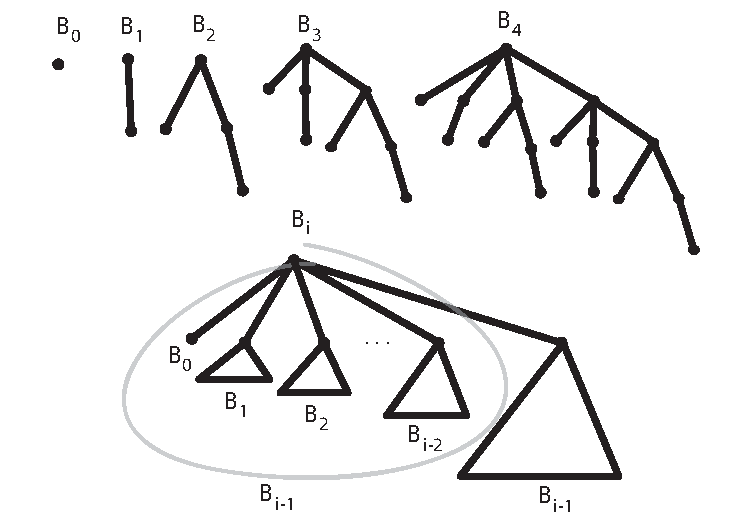
\includegraphics{pics/binheaps}
\caption{Binomiální stromy}
\label{fig.heaps.binomial}
\end{figure}

\begin{tvrzeni}
Binomiální halda je tvořena binomiálními stromy $B_i$, které mají následující
vlastnosti: 
\begin{itemize}
\item $B_i$ má $2^i$ vrcholů
\item hloubka $B_i$ je i
\item kořen $B_i$ má i synů
\item $\forall j < i$ existuje syn kořene $B_i$ takový, že 
  jeho podstrom je izomorfní s $B_j$.
\end{itemize}
\end{tvrzeni}

\begin{proof}
indukcí přes $i$ (elementární)
\end{proof}


\subsection{MERGE}

Algoritmus MERGE (viz algoritmus \ref{alg:heaps.binom.merge}) pracuje jako
"binární sčítání" - 2 stromy $B_i$ (= 2 jedničky v řádu $i$) slije do
$B{i-1}$ (= přenos do $i+1$)

Pracuje v $O(\log_2 n)$ - nejvyšší možný řád je $\lfloor \log_2 n \rfloor$.
Toto je složitost v nejhorším případě.

Ukazatel MIN nové haldy je nastaven na menší z MIN($h_1$), MIN($h_2$) - to
zabere $O(1)$.


\begin{algorithm}[!htb]
\caption{MERGE pro binomiální haldy}
\label{alg:heaps.binom.merge}
\begin{algorithmic}
\STATE MERGE($T_1$, $T_2$)
\STATE ($T_1, T_2$ binom. haldy velikosti $n_1,n_2$)
\STATE $P = 0, i = 0, T = 0$
\WHILE {$i \leq log(n_1 + n_2)$}
  \STATE $S_1$ je strom v $T_1$ izomorfní s $H_i$ (pokud neexistuje, tak $S_1=0$)
  \STATE $S_1$ je strom v $T_1$ izomorfní s $H_i$ (pokud neexistuje, tak $S_1=0$)
  % XXX \CASE
     \IF {$S_1, S_2$, P = 0}
       \STATE neprovedeme nic
     \ENDIF
     \IF {jeden strom z $S_1, S_2$, $P$ je neprázdný} 
        \STATE vložím tento strom do $T$, $P=0$
     \ENDIF
     \IF {dva stromy z $S_1, S_2$, $P$ jsou neprázdné}
       \STATE spojím tyto stromy a výsledek vzložím do $P$
     \ENDIF
     \IF {všechny stromy z $S_1, S_2$, $P$ jsou neprázdné}
       \STATE vložím do $T$, spojení $S_1, S_2$ vložím do $P$
     \ENDIF
  % \ENDCASE
  \STATE $i = i + 1$
\ENDWHILE
\end{algorithmic}
\end{algorithm}

\begin{pozn}
V algoritmu MERGE (viz algoritmus~\ref{alg:heaps.binom.merge}) 
odpovídá $P$ přenosu v binárním sčítání, $T$ je výsledná halda.
\end{pozn}

\subsection{MIN}

MIN($h$) - prohledáme prvky reprezentované kořeny stromů a najdeme
nejmenší. V praxi je pro každou haldu držen ukazatel, ukazující na kořen
reprezentující nejmenší prvek haldy. Tento ukazatel je obnovován při
operaci DELETE\_MIN.


\subsection{INSERT}

Operace INSERT($h$,$i$) se provede příkazem MERGE($h$, MAKEHEAP($i$)).
Tato operace je analogická s inkrementací binárního čítače.

Dijkstrův algoritmus provádí na začátku $n$ operací INSERT, nám tedy nejde
o jednotlivé operace, ale o posloupnost INSERTů.

\begin{pozn}
INSERT je stejný jako v leftist haldách.
\end{pozn}

\begin{theorem}
Amortizovaná složitost operace INSERT je $O(1)$.
\end{theorem}

\begin{proof}
Využijeme účetní metody: \\
Algoritmus INSERT udržuje následující invariant: \\
Každý binom. strom v haldě má na svém účtu 1 jednotku. (Ten, který
přestává být kořenem, zaplatí, ten kdo vyhrál, si 1 jednotku ponechal.)
Při vytváření stromu ji zaplatí operace, která strom vytvořila: 
\begin{itemize}
  \item MAKEHEAP vytvoří 1 strom $\Rightarrow$ zaplatí 1
  \item DELETE\_MIN vytvoří $\leq log n$ stromů $\Rightarrow$ zaplatí
  	$\leq log n$
\end{itemize}
Pokud INSERT spustí kaskádu slévání, pak je každé slití zaplaceno z účtu
stromu, který daným slitím zanikne. (jeho kořen se stane synem)
\end{proof}


\subsection{DELETEMIN}

Operace DELETEMIN (viz algoritmus \ref{alg:heaps.binom.deletemin}) 
je provedena tak, že ze stromu $B_k$, na který ukazuje
ukazatel MIN, utrhneme kořen. Tím vzniknou nové stromy $B_0, B_1, ...,
B_{k-1}$, ze kterých vytvoříme novou haldu, nastavíme pro ni ukazatel MIN
a zavoláme MERGE.

DELETEMIN pracuje v $O(log_2 n)$, protože $k \leq log_2 n$. Toto je
složitost v nejhorším případě.

\begin{algorithm}[!htb]
\caption{DELETEMIN pro binom. haldu}
\label{alg:heaps.binom.deletemin}
\begin{algorithmic}
\STATE DELETEMIN
\STATE prohledáním prvků reprezentovaných kořeny stromů naleznu strom $S$,
jehož kořen reprezentuje nejmenší prvek
\STATE $T_1 = T \ {S}, T_2$ je tvořen podstormy všechn synů kořene S
\STATE (tj. utrhnu kořen a zbytek dám do haldy) - 
	je to halda díky vlastnosti 4
\STATE $T \rightarrow$ MERGE($T_1, T_2$)
\end{algorithmic}
\end{algorithm}

\begin{pozn}
Operace DELETE se nedá rozumně provést, museli bychom přebudovat celý
strom.
\end{pozn}

\begin{theorem}
Operace MERGE, INSERT, MIN, DELETEMIN a DECREASEKEY vyžadují čas $O(log n)$.
Operace INCREASEKEY vyžaduje čas $O(log^2 n)$.
\end{theorem}

%\begin{pozn}
%Sčítání v binárních číslech má složitost $O(1)$.
%
%\begin{tabular}{|l|}
%\hline
%1 0 0 ... 0 \\
%\hline
%1 1 1 ... 1 \\
%\hline
%\end{tabular}
%\hspace{5mm}
%
%XXX amort. slož. \\
%Neplatí něco podobného pro binom. stromy ? Ano, pro operaci INSERT.
%\end{pozn}

\begin{pozn}
MERGE zabírá dost času - musíme ho dělat ?
\end{pozn}


\subsection{Líná implementace binom. hald}

Líná implementace vychází z toho, že chceme operaci MERGE provádět v čase
$O(1)$.

Změníme definici - vynecháme podmínku 2 z definice \ref{def.binomheap}, 
tj. teď v naší binom. haldě mohou být izomorfní stromy. (i když jen
dočasně) Další změna
spočívá ve změně reprezentace binomiální haldy - haldu reprezentujeme
dvojitým kruhovým spojovým seznamem přes kořeny stromů. (kruhový spojový
seznam umožňuje přidávání a odebírná prvků v čase $O(1)$.)

Operaci MERGE($T_1, T_2$) pak můžeme provést konkatenací seznamů $T_1$ a $T_2$.
Jenom to by nefungovalo, musíme ještě změnit operace MIN, DELETEMIN.

\begin{algorithm}[!htb]
\caption{DELETEMIN pro líné binom. haldy}
\label{alg:heaps.binom-line.min}
\begin{algorithmic}
\STATE MIN
\STATE při prohledávání prvků reprezentovaných kořeny stromů seřadíme
stromy do množin $Q_i$, $i=0,...,n$ , kde $Q_i$ je množina všech stromů v
$T$ izomorfních s $B_i$.
\STATE $i = 0, T = 0$
\WHILE {$\exists Q_i \neq 0$}
  \WHILE {$|Q_i| > 1$}
    \STATE vezmeme dva stromy z $Q_i$, spojíme je, výsledek dáme do $Q_{i+1}$
  \ENDWHILE
  \IF {$Q_i \neq 0$}
    \STATE strom z $Q_i$ dám do $T$
  \ENDIF
  \STATE $i = i + 1$
\ENDWHILE
\end{algorithmic}
\end{algorithm}

DELETEMIN umístí stromy po odtržení nejmenšího prvku do odpovídajících 
množin $Q_i$. (v množině $Q_i$ jsou stromy izomorfní s $B_i$)
Poté provede \emph{konsolidaci} - upraví haldu do podoby, kdy je každý řád
zastoupen nejvýše jedním stromem. 

Konsolidace běží v $O(log n)$ plus vyčerpá účty stromů, které zaniknou při
slévání.

\begin{samepage}
Konsolidace probíhá takto:
\begin{enumerate}
  \item vytvořím pole délky $log n$, které je prázdné 
  	$\Rightarrow$ $O(log n)$
  \item procházím spojový seznam vrcholů stromů v haldě 
  	a jeden strom za druhým vyjmu a 
  	dávám do pole vytvořeného v kroku 1, přičemž se vždy provede 
	příslušné slití.
	\begin{itemize}
	  \item pokud strom zanikne, tak práci zaplatíme z jeho účtu
	  \item pokud strom nezanikne, tak práci platíme z účtu
	  konsolidace $\rightarrow$ $O(log n)$
	\end{itemize}
  \item z pole vytvoříme spojový seznam $\rightarrow$ $O(log n)$
\end{enumerate}
\end{samepage}

\begin{samepage}
DELETEMIN tedy potřebuje
\begin{itemize}
  \item $O(log n)$ do účtů nově vytvořených stromů
  \item $O(log n)$ na jejich zavedení do spojového seznamu
  \item $O(log n)$ na konsolidaci
\end{itemize}
\end{samepage}

Při konsolidaci vždy zároveň vyhledáme nové minimum.

\begin{theorem}
Operace MERGE a INSERT při líné implementaci vyžadují čas $O(1)$, operace
DELETEMIN a MIN vyžadují čas $O(\text{počet stromů v haldě})$.
\end{theorem}

%\begin{pozn}
%$bal(\text{konfigurace}) = \text{počet všech stromů ve všech haldách v
%konfiguraci}$
%\end{pozn}
%
%\subsubsection{Amort. slož.}
%$\text{amort. slož.} = \text{čas pro operaci} + 
%bal(\text{výsledné konfigurace}) - bal(\text{původní konfigurace})$

\vspace{5mm}

\begin{center}
\begin{tabular}{|l|l|}
\hline
Operace & Amort. složitost \\
\hline
MERGE & $O(1)$ \\
INSERT & $O(1)$ \\
MIN & $O(log n)$ \\
DELETEMIN & $O(log n)$ \\
\hline
\end{tabular}
\tabcaption{Amortizovaná složitost pro líné binomiální haldy}
\label{tab:binheaps.lazy.complexity}
\end{center}

% \subsection{Zobecněné binomiální haldy}

% XXX
% \mnote{přednášelo se to tento rok (2004) vůbec ?}

% --------------------------------------------------------------------------
\section{Fibonacciho haldy}

Fibonacciho haldy vycházejí z binomiálních hald, formálně se liší v podstatě
pouze tím, že v haldě povolíme i jiné stromy než binomiální. Toto nám
umožní implementaci operace DECREASE\_KEY, která nebyla v binomiálních
haldách při zachování složitosti ostatních operací možná.

Řád uzlu a stromu je definován jako u binomiálních hald. Slévání se
provádí pouze mezi stromy stejného řádu.

\subsection{MERGE, INSERT, EXTRACT\_MIN}

Implementace operací MERGE($h_1$,$h_2$), INSERT($h$,$i$), EXTRACT\_MIN($h$) 
je stejná jako u binomiálních hald v "líné" verzi.

\subsection{DECREASE\_KEY}

DECREASE\_KEY provádí snížení hodnoty klíče pro daný prvek. To se děje za
cenu přítomnosti jiných než binomiálních stromů v haldě.

\begin{algorithm}[!htb]
\caption{DECREASE\_KEY pro Fibonacciho haldy}
\label{alg:heap.fib.decrease_key}
DECREASE\_KEY($h$,$i$,$\delta$)
\begin{enumerate}
  \item snížím klíč prvku $i$ o $\delta$
  \item podstrom i s kořenem $i$ odřízneme a jako samostatný strom ho
        zavedeme haldy (tj. zařadím do spojového seznamu kořenů stromů v
	haldě) $\Rightarrow$ $O(1)$
  \item Abychom udrželi stromy dostatečně "košaté"\footnote{nechceme 
  	stromy typu "smeták" - tj. takových, které sestávají pouze 
	z kořene a jeho synů, které jsou zároveň listy}
  	tak od každého vrcholu $x$ mohou být odříznuti nejvýše 2
  	synové $\Rightarrow$ po odříznutí 2. syna je odříznut i sám vrchol $x$.
\end{enumerate}
\end{algorithm}

\begin{figure} 
\centering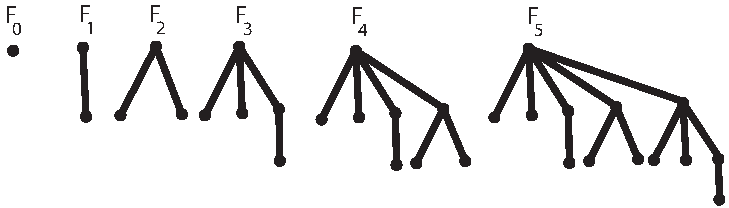
\includegraphics{pics/fibheaps}
\caption{Počty vrcholů stromů $F_0, F_1, ...$ tvoří Fibonacciho
posloupnost.}
\label{fig:heaps.fib.pocty.vrcholu}
\end{figure}

\begin{pozn}
Přestože jedna operace DECREASE\_KEY může vyvolat kaskádu řezů, je její
amortizovaná složitost $O(1)$.
\end{pozn}

\begin{pozn}
Pomocí \emph{účetní metody}\footnote{Pro definici účetní metody viz
přednášky ze "\emph{Složitosti a NP úplnosti}".}
dokážeme, že to platí: \\
Při odřezávání syna vrcholu $x$ zaplatí operace DECREASE\_KEY
\begin{samepage}
\begin{itemize}
  \item 2 jednotky na účet $x$
  \item 1 jednotku na účet vzniklého stromu
  \item 1 jednotku za práci (odříznutí a zařazení)
\end{itemize}
\end{samepage}

Při odříznutí druhého syna jsou na účtu vrcholu $x$ 4 jednotky
$\Rightarrow$ mohu zopakovat body 1) - 3).
\end{pozn}

\begin{theorem}
\label{heaps.fib.theorem}
Nejvyšší řád stromu ve Fibonacciho haldě je $\lfloor log_\varphi n \rfloor =
\Theta(log_2 n)$ pro nějaké $\varphi > 1$.
\end{theorem}

\begin{lemma}
\label{heaps.fib.lemma}
Nechť $x$ je vrchol a $y_1, ..., y_m$ jeho synové v pořadí, v jakém byli k
$x$ sliti. Potom $\forall \in {1,...,m}$ je řád $y_i$ aspoň $i-2$.
\end{lemma}

\begin{proof}
V okamžiku, kdy byl $y_i$ slit pod $x$, měl $x$ řád $\geq i-1$.
($y_1,...,y_{i-1}$ již v té chvíli byli synové $x$)
V tomto okamžiku byl také řád $y_{i-1} \geq i-1$. (sléváme pouze stromy
stejného řádu) Od té doby mohl $y_i$ ztratit nejvýše jednoho syna, jinak
by byl sám odříznut a přestal by být synem $x$. $\Rightarrow$ $y_i$ má řád
$\geq i-2$. 
\end{proof}

\begin{proof}
Dokazujeme větu \ref{heaps.fib.theorem}, která jinými slovy říká: 
Strom řádu $i$ ve
Fibonacciho haldě má velikost alespoň $\varphi^i$ pro nějaké $\varphi >
1$.

Nechť $F_j$ je nejmenší možný (tj. má ořezané podstromy na max. možnou
úroveň - byl z nich odříznut 1 syn) strom řádu $j$ splňující tvrzení lemma
\ref{heaps.fib.lemma} a nechť $|F_j| = f_j$. Pak

\begin{enumerate}
  \item $F_i$ vznikne "slitím" $F_{i-1}$ a $F_{i-2}$ $\Rightarrow$ 
  	$f_i = f_{i-1} + f_{i-2}$
  \item $f_i \geq \varphi^i$, kde 
  	$\varphi = \frac{1+\sqrt 5}{2} \approx 1.618$ ... zlatý řez
\end{enumerate}

\begin{itemize}
  \item[ad 1)] 
  viz obr.~\ref{fig:heaps.fib.proof}

  \begin{figure} 
  \centering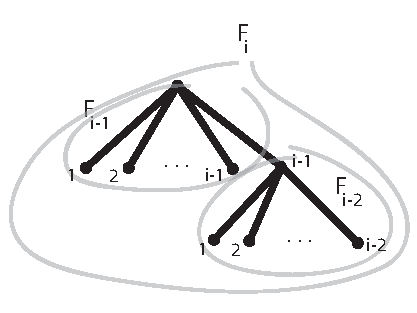
\includegraphics{pics/fibheap}
  \caption{K důkazu věty \ref{heaps.fib.theorem}}
  \label{fig:heaps.fib.proof}
  \end{figure}

  Slití je nepřesný termín - sléváme pouze stromy stejného řádu.
  $F_{i-2}$ je výsledek DECREASE\_KEY. (tím se strom "oholil") Uříznu
  posledního syna, pod kterým je největší podstrom (abych dostal nejmenší
  možný podstrom)

  \item[ad 2)]
  $\varphi$ je kladý kořen rovnice $x^2 - x - 1 = 0$ \\
  neboli platí $\varphi^2 = \varphi + 1$, $\varphi = \frac{1+\sqrt 5}{2}
  \approx 1.618$ \\
  dokážeme indukcí: 
    \begin{itemize}
      \item i = 0 : $f_0 = 1 \geq \varphi^0 = 1$
      \item i = 1 : $f_1 = 2 \geq \varphi^1 = 1.618$
      \item indukční krok: IP: $f_i \geq \varphi^i$, $f_{i+1} \geq
      \varphi^{i+1}$ \\
        $f_{i+2} = f_{i+1} + f_i \geq \varphi^{i+1} + \varphi^i =
	\varphi^i(\varphi + 1) = \varphi^{i+2}$
    \end{itemize}
\end{itemize}
\end{proof}


